\documentclass[11pt]{article}

\usepackage{amsmath}
\usepackage{amsfonts}
\usepackage[margin=1in]{geometry}
\usepackage{enumitem}
\usepackage{graphicx}
\usepackage[colorlinks]{hyperref}
\usepackage{longtable}

\usepackage{helvet}
\renewcommand{\familydefault}{\sfdefault}

\setlength{\parindent}{0in}

\def\tightlist{}
\def\toprule{}
\def\bottomrule{}

\begin{document}
{\LARGE Homework 6 (Due October
21st)}\label{homework-6-due-october-21st}\\

{\Large 1. Method of Relaxation for Cartesian
Problems}\label{method-of-relaxation-for-cartesian-problems}

One of the major properties of a solution to Laplace's equation is that
the value of the potential at a point is equal the average of all the
points surrounding it (i.e., a sphere in 3D or a circle in 2D). We can
exploit this property to solve Laplace's equation numerically by
successively computing the average value of the potential at a point on
a mesh (a grid of 2D points in this case) based on the 4 other points
that surround it (see the figure below).

\begin{figure}[htbp]
\centering
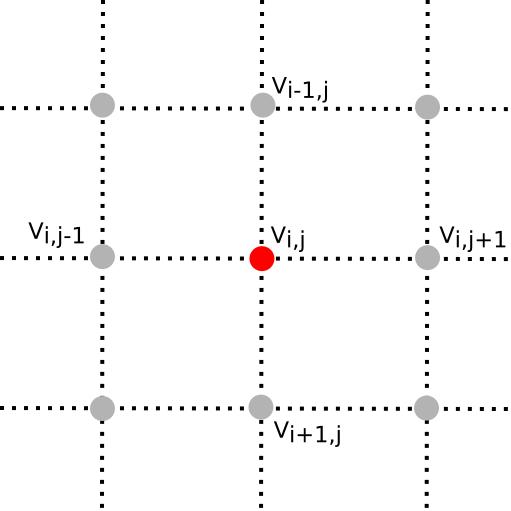
\includegraphics[width=0.5\linewidth]{./images/hw6/mesh.png}
\end{figure}

To be explicit, in the simplest relaxation codes, which can run for an
inordinate amount of time given the size of the mesh and the error
tolerance demanded, we replace the value of the potential \(V_{i,j}\)
with the arithmetic average of its closest neighbors on the mesh:

\[V_{i,j} = \dfrac{1}{4}\left(V_{i-1,j} + V_{i,j-1} + V_{i,j+1} + V_{i+1,j}  \right)\]

The procedure for solving Laplace's equation numerically involves the
following steps:

\begin{itemize}
\tightlist
\item
  \textbf{Step 1:} Slice up the space where \(\nabla^2 V = 0\) (and the
  boundary) into a grid of points (called a ``mesh'') that are spaced an
  equal distance apart. \emph{That mesh may have different spacing
  between points based on what the details of the problem being solved
  might be. For example, if the potential is expected to be change over
  short distances in some points and not others, it can make sense to
  change the spacing to optimize computational time (or memory).} In
  this problem, we will use a mesh of equally spaced points.
\item
  \textbf{Step 2:} Set the value of the boundary points given the
  specific problem you intend to solve. \emph{This will typically be
  done in the initial parts of the program and can be changed easily to
  solve other kinds of problems.} In this problem, we will start with a
  non-zero constant value (10 V) on one edge and zero at the other 3
  edges.
\item
  \textbf{Step 3:} Starting at some location away from the boundary,
  systematically loop through each point applying the averaging function
  given above. \emph{It would be typical to start at one corner of the
  mesh and move systematically across (or down) and then down (or
  across) calculating the value at each new point as you go.}
\item
  \textbf{Step 4:} Compute the difference between the starting values of
  the potential and the values after a full iteration. Compare this
  difference to the accepted error that you decided on before starting
  the calculation, \(Error_{i,j} = Vnew_{i,j}-Vold_{i,j}\). \emph{Here,
  you could use the average error, the maximum error, or something
  else.} In this problem, you will use the maximum error on the mesh,
  which we will set (at first) to 1e-1.
\item
  \textbf{Step 5:} Repeat steps 3 and 4 until the computed error is
  below the accepted error.
\item
  \textbf{Step 6:} Plot the results as either a 3D plot or a contour map
  (or both). In this problem, you will be asked to produce both plots.
\end{itemize}

So for this problem,
\href{../jupyter/HW6-MethodOfRelaxation.ipynb}{download this Jupyter
notebook} (you can
\href{https://github.com/dannycab/phy481msu/blob/gh-pages/jupyter/HW6-MethodOfRelaxation.ipynb}{view
it here}), which sets up most of the aspects of the problem.

\begin{enumerate}
\def\labelenumi{\arabic{enumi}.}
\tightlist
\item
  Identify where in the code steps 1-3 above are occurring. Explain what
  each line of code that perform steps 1-3 are doing.
\item
  Determine where the averaging and error checking must occur in the
  code and add the lines needed to do these computation. \emph{Hint:
  there's only two lines to add and both of them are written as regular
  math above. It's your job to figure out where the go and how they are
  written.}
\item
  Produce a 3D Plot of the potential. You did this with
  \href{./homework6.html}{a problem on the last homework}.
\item
  \href{http://matplotlib.org/examples/pylab_examples/contour_demo.html}{Review
  how to make a contour plot using matplotlib} and produce a contour
  plot of your results.
\item
  Determine how many iterations on the mesh (\emph{look for the print
  statements at the end of the code}) are needed to obtain an error
  tolerances of: 1e-2, 1e-3, 1e-4, 1e-5, 1e-6, and 1e-7. \emph{You might
  have to adjust the maximum number of iterations as the error tolerance
  is decreased.}
\item
  \textbf{BONUS (Worth up to 2 parts of 1 problem):} Set the value of
  the boundary to something more interesting (your choice!) and repeat
  parts 2 and 3.
\end{enumerate}

{\Large 2. Sphere with a known
potential}\label{sphere-with-a-known-potential}

We have a sphere (radius, \(R\)) where we have glued charges to the
outside such that the electric potential at the surface of the sphere is
given by:

\[V_0 = k \cos 3\theta\]

where \(k\) is some constant.

You are going to find the potential inside and outside the sphere (there
are no charges other than those at the surface of the sphere) as well as
the charge density \(\sigma(\theta)\) on the surface of the sphere. Each
part of this problem is meant to walk you through the process for
solving these kinds of boundary-value problems.

\begin{enumerate}
\def\labelenumi{\arabic{enumi}.}
\tightlist
\item
  Rewrite the potential at the surface using Legendre polynomials.
  \emph{You will need to dust off some trig identities to do this.}
\item
  Using this boundary condition and the knowledge that \(V\) should be
  finite inside the sphere, find the electric potential,
  \(V(r,\theta)\), inside this sphere. You do not have to re-derive the
  general solution to Laplace's equation, just use the result:
  \[V(r,\theta) = \left(A_lr^l+\dfrac{B_l}{r^{l+1}}\right)P_l(\cos \theta)\]
\item
  Using the same boundary condition and the knowledge that \(V\) should
  vanish far from the sphere, find the electric potential,
  \(V(r,\theta)\), outside this sphere.
\item
  Show explicitly that your solutions to parts 2 and 3 match at the
  surface of the sphere.
\item
  Take the ``normal'' derivative of each of your solutions
  (\(\partial V/\partial r\)) and use their difference at the surface to
  find the charge on the surface:
  \[\left(\dfrac{\partial V_{out}}{\partial r}-\dfrac{\partial V_{in}}{\partial r}\right) = -\dfrac{\sigma}{\varepsilon_0}\]
\item
  Sketch the charge distrbution on the surface of the sphere.
\end{enumerate}

{\Large 3. Solving Laplace's Equation in Cylindrical
Coordinates}\label{solving-laplaces-equation-in-cylindrical-coordinates}

We have gone through how to solve Laplace's equation in Cartesian and
spherical coordinates. In both cases, finding a separable and general
solution was possible. In fact, there are a
\href{http://mathworld.wolfram.com/LaplacesEquation.html}{number of
possible coordinate systems} where we can do this, but the most relevant
to this class (besides Cartesian and spherical) is cylindrical
coordinates.

In this problem, you will develop the general solution to Laplace's
equation in cylindrical coordinates where there is no dependence on the
\(z\) coordinate (i.e., where we have cylindrical symmetry).

\begin{enumerate}
\def\labelenumi{\arabic{enumi}.}
\tightlist
\item
  Starting from Laplace's equation in Cylindrical coordinates, use the
  ansatz \(V(s,\phi) = S(s)\Phi(\phi)\) to convert the problem from one
  partial differential equation to two 2nd order ordinary differential
  equations -- one for \(S(s)\) and one for \(\Phi(\phi)\).
\item
  As we have argued twice, each of those differential equations is equal
  to a constant. Which constant is positive and which is negative?
  Explain your choice. \emph{Think about what happens when you rotate
  your problem by 2\(\pi\) in the \(\phi\) direction, should the physics
  care that you've done that?} Going forward, choose the positive
  constant to be \(+k^2\) and the negative one to be \(-k^2\).
\item
  Solve the differential equation for \(\Phi(\phi)\) to obtain the
  general solution for \(\Phi(\phi)\). Hint:
  \(\Phi(\phi) = \Phi(\phi + 2\pi)\) so this puts an additional
  condition on \(k\) that it must be an integer with \(k \geq 0\).
\item
  Armed with this information about \(k\), solve the differential
  equation for \(S(s)\) to obtain the general solution for \(S(s)\).
  \emph{Be careful to treat \(k=0\) separately as that generates an
  additional and completely physical solution!}
\item
  The potential at a distance \(s\) away from an infinite line charge
  (which should be captured by this solution) is:
  \(V(s) = \dfrac{2\lambda}{4 \pi\varepsilon_0}\ln(s)\) + constant,
  which terms in general solution vanish to capture this solution?
\end{enumerate}

\emph{This problem is tough. But here's a little help. The general
solution for the electric potential in cylindrical coordinates (with
cylindrical symmetry) is:}

\[V(s,\phi) = a_0 + b_0 \ln s + \sum_{k=1}^\infty \left[s^k(a_k \cos k\phi + b_k \sin k \phi)+s^{-k}(c_k \cos k\phi + d_k \sin k \phi)\right]\]

You will not get full credit for this problem unless your work clearly
shows how you this solution is developed.

{\Large 4. Zen and the Art of the Multipole
Expansion}\label{zen-and-the-art-of-the-multipole-expansion}

Developing intuition about the dominant contribution to the field that
you are looking at will serve you very well in the future. In this
problem, you will look at a few charge distributions (blue - positive
charge; orange - negative charge) and discuss what the dominant
contribution (monopole, dipole, quadrapole) to the field would be far
from the distribution (as \(r \rightarrow \infty\)).

For each distribution below, discuss which contribution to the multipole
expansion dominants at large \(r\). Explain how you can tell this is the
dominant contribution (use equations, pictures, and words as you see
fit).

\begin{enumerate}
\def\labelenumi{\arabic{enumi}.}
\tightlist
\item
  Distribution 1: 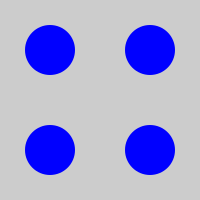
\includegraphics[width=0.2\linewidth]{./images/hw6/distribution1.png}
\item
  Distribution 2: 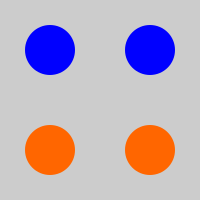
\includegraphics[width=0.2\linewidth]{./images/hw6/distribution2.png}
\item
  Distribution 3: 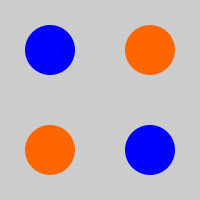
\includegraphics[width=0.2\linewidth]{./images/hw6/distribution3.png}
\end{enumerate}

{\Large 5. The Beauty of the Multipole
expansion}\label{the-beauty-of-the-multipole-expansion}

The \href{https://en.wikipedia.org/wiki/Multipole_expansion}{multipole
expansion} is a very powerful approximation that arises in a number of
different kinds of field theories. The beauty of it is that it can
provide a simple approximate form for the field in question far from the
sources that produce the field. Often, this is helpful when solving
problems where you only care about the dominant contributions because
the others only provide small corrections to the behavior.

In this problem, you will explore the the multipole expansion for the
charge configuration shown below.

\begin{figure}[htbp]
\centering
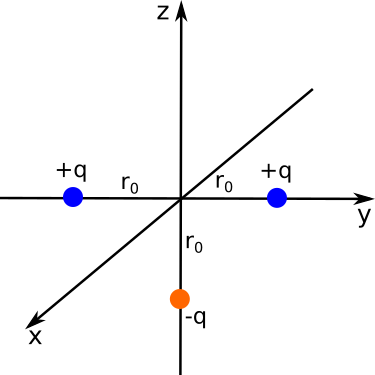
\includegraphics[width=0.5\linewidth]{./images/hw6/multipole.png}
\end{figure}

\begin{enumerate}
\def\labelenumi{\arabic{enumi}.}
\tightlist
\item
  For the three charges shown above, determine the approximate potential
  at a distance far from the origin of coordinates. Keep only the two
  lowest non-vanishing orders of the expansion. \emph{Notice that each
  is a distance \(r_0\) from the origin.}
\item
  Explain how you know the two terms you find are the lowest
  non-vanishing terms for the potential.
\item
  Using your answer to part 1, find the approximate electric field
  produced by this system of charges far from the origin. Express your
  answer in spherical coordinates.
\end{enumerate}
\end{document}
